%% A Confidence-Tiered AI Pipeline for Phishing Website Detection
%% IEEE conference draft (IEEEtran). Compile with pdfLaTeX + BibTeX:
%%   pdflatex phishing_tiered_ai_draft
%%   bibtex   phishing_tiered_ai_draft
%%   pdflatex phishing_tiered_ai_draft
%%   pdflatex phishing_tiered_ai_draft
%% The Vietnamese abstract uses UTF-8 + T5 font encoding under pdfLaTeX.
%% If diacritics do not render, compile with XeLaTeX or LuaLaTeX instead
%% (remove the inputenc/fontenc lines and add \usepackage{fontspec}).
%%
%% STATUS: system-design and evaluation-protocol paper. No empirical results
%% for the proposed system are reported. Cited quantitative values are sourced;
%% "target"/"budget" values are design goals; "preliminary inspection" values
%% are the authors' own observations on the public training file.

\documentclass[conference]{IEEEtran}
\IEEEoverridecommandlockouts

\usepackage[utf8]{inputenc}
\usepackage[T5,T1]{fontenc}
\usepackage{cite}
\usepackage{amsmath,amssymb}
\usepackage{graphicx}
\usepackage{url}
\usepackage{hyperref}
\usepackage{textcomp}
\usepackage{xcolor}
\usepackage{booktabs}
\usepackage{tikz}
\usetikzlibrary{arrows.meta,positioning,shapes.geometric}

\begin{document}

\title{A Confidence-Tiered AI Pipeline for Phishing Website\\ Detection and Warning, with a Vietnamese\\ Brand-Impersonation Focus}

\author{
\IEEEauthorblockN{[Author 1] and [Author 2]}
\IEEEauthorblockA{[Faculty of Information Technology, University Name], Vietnam\\
Email: dongquan2110@gmail.com}
}

\maketitle

\begin{abstract}
Phishing detection systems increasingly combine a lightweight machine-learning
(ML) classifier with a large language model (LLM) for deep analysis, but most
designs invoke the LLM for every request that needs scrutiny, and virtually all
published systems are built and evaluated on English-language brands. We present
the design of a confidence-tiered pipeline that spends heavy analysis only where
it is warranted and that treats Vietnamese brand impersonation as a first-class
concern. Layer~A is a Manifest~V3 \texttt{declarativeNetRequest} blocklist that
blocks known-bad domains instantly and grows itself from confirmed downstream
verdicts. Layer~B extracts the 87 features of the Hannousse--Yahiouche benchmark
dataset, scores them with a Random Forest, and runs three override rules in
parallel: domain age via RDAP with a WHOIS fallback, TLS-certificate validity and
recency, and Levenshtein typosquatting distance against a curated list of
Vietnamese brand domains. A URL passes immediately only if the Random Forest
score is low \emph{and} no override rule fires; every other case enters a single
``suspicious zone,'' where a locally hosted small model of the Qwen3.5 family
($\approx$2\,B parameters, e.g.\ \texttt{qwen3.5:2b}), grounded by a two-tier
retrieval-augmented generation (RAG) store, produces the final verdict and a
human-readable explanation, and any domain it confirms malicious is written back
into Layer~A. We motivate each choice against the literature, give a simple cost
model for why self-hosted inference removes the incentive to split ``grey'' and
``black'' LLM tiers, and analyze the LLM stage's security exposure with the OWASP
Top~10 for LLM Applications~(2025). We close with a pre-registered evaluation
protocol. \emph{No results for the proposed system are reported here; this paper
specifies an architecture and a measurement plan.}
\end{abstract}

\begin{IEEEkeywords}
phishing detection, machine learning, large language models, retrieval-augmented
generation, browser extension, Manifest~V3, prompt injection, Vietnamese brand
impersonation.
\end{IEEEkeywords}

\section*{Tóm tắt (Vietnamese abstract)}
Các hệ thống phát hiện lừa đảo (phishing) hiện nay thường kết hợp bộ phân loại
học máy nhẹ với mô hình ngôn ngữ lớn (LLM) để phân tích sâu, nhưng phần lớn thiết
kế gọi LLM cho \emph{mọi} yêu cầu cần xem xét, và gần như toàn bộ hệ thống đã công
bố đều dựa trên thương hiệu tiếng Anh. Bài báo trình bày thiết kế một pipeline
phân tầng theo độ tin cậy: chỉ dồn phân tích sâu vào phần traffic thật sự đáng
ngờ, và đặt bối cảnh giả mạo thương hiệu Việt Nam làm trọng tâm. Lớp~A là
blocklist \texttt{declarativeNetRequest} (Manifest~V3) chặn tức thì domain đã
biết xấu và tự học từ phán quyết được xác nhận ở lớp sau. Lớp~B trích 87 đặc
trưng của bộ dữ liệu chuẩn Hannousse--Yahiouche, chấm điểm bằng Random Forest,
đồng thời chạy song song ba luật: tuổi domain qua RDAP (dự phòng WHOIS), tính hợp
lệ và độ mới của chứng chỉ TLS, và khoảng cách Levenshtein so với danh sách domain
thương hiệu Việt Nam. Một URL chỉ được cho qua ngay khi điểm Random Forest thấp
\emph{và} không luật nào kích hoạt; mọi trường hợp còn lại vào ``vùng nghi ngờ''
duy nhất, nơi một mô hình nhỏ thuộc họ Qwen3.5 ($\approx$2 tỷ tham số, ví dụ
\texttt{qwen3.5:2b}) chạy cục bộ, tăng cường bằng kho RAG hai tầng, đưa ra phán
quyết cuối cùng kèm giải thích; domain bị xác nhận nguy hiểm được nạp ngược vào Lớp~A. Chúng tôi lập
luận cho từng lựa chọn thiết kế dựa trên tài liệu, đưa ra một mô hình chi phí đơn
giản giải thích vì sao suy luận tự host loại bỏ động lực tách hai mức LLM, và phân
tích rủi ro bảo mật của tầng LLM theo OWASP Top~10 for LLM Applications~(2025).
Bài báo kết thúc bằng một giao thức đánh giá đăng ký trước. \emph{Bài báo không
báo cáo kết quả thực nghiệm của hệ thống đề xuất.}

\medskip
\noindent\textbf{Từ khóa:} phát hiện phishing, học máy, mô hình ngôn ngữ lớn, RAG,
tiện ích trình duyệt, Manifest~V3, prompt injection, giả mạo thương hiệu Việt Nam.

\section{Introduction}
Phishing remains one of the highest-volume forms of online fraud. Recent surveys
report that machine-learning approaches now dominate phishing-website
detection~\cite{safi2023slr,divakaran2022review}, and a hybrid arrangement has
become common in practice: a fast statistical model filters the bulk of traffic
and a slower, more expressive model resolves the hard
cases~\cite{koide2024chatphishdetector,divakaran2022review}. Two limitations
recur.

\emph{First, the expensive stage is invoked too often.} Systems that use an LLM
as the deep analyzer typically call it for every input the fast stage cannot
dismiss~\cite{koide2024chatphishdetector,lee2024multimodal}. When the LLM is a
paid cloud API, this couples detection coverage directly to operating cost, and
it is the reason several designs add a cheaper ``grey-zone'' model before
escalating.

\emph{Second, the evaluation context is almost entirely English.} The datasets
and brand lists used by the surveyed literature~\cite{koide2024chatphishdetector,
lee2024multimodal,hannousse2021benchmark,tamal2024ofva} are built on
internationally known, English-language brands. Vietnamese banking, e-commerce,
and e-wallet brands---the actual impersonation targets for Vietnamese users---are
absent.

This paper describes a pipeline organized by \emph{confidence tiering}: classify
each URL by how certain the system is, and let that certainty decide how much
computation the URL receives. Three defensive layers run before any generative
model is consulted: (1)~Layer~A blocks already-known malicious domains using the
browser's native \texttt{declarativeNetRequest} mechanism and extends its own
blocklist from verdicts confirmed later; (2)~Layer~B combines a Random Forest
over the 87-feature Hannousse--Yahiouche
representation~\cite{hannousse2021benchmark,hannousse2021dataset} with three
parallel override rules; (3)~the suspicious zone is reached only when Layers~A
and~B are jointly inconclusive, and there a locally hosted small LLM grounded by a
two-tier RAG store issues the final verdict and an explanation. Two of these are
deliberate design choices rather than novel mechanisms: requiring the statistical
score \emph{and} the technical rules to agree before the cheap path is taken (a
stricter gate than a plain fast/slow cascade), and merging the customary
grey/black LLM split into one zone because self-hosted inference has no
per-request price to control (Section~\ref{sec:rationale}).

\emph{Contributions.} (i)~A concrete instantiation of a tiered detector for
\textbf{Vietnamese brand impersonation} --- the two-tier RAG design, the curated
brand-domain table, and the three override rules; (ii)~a security analysis of the
LLM stage mapped to the OWASP Top~10 for LLM Applications~(2025)~\cite{owasp2025llmtop10},
including a shared-blocklist self-poisoning risk we have not seen discussed
elsewhere; (iii)~a design-rationale analysis, with a simple cost model, tying
each choice to the literature and to consumer-grade hardware constraints; and
(iv)~a pre-registered evaluation protocol with fixed numeric targets and
pass/fail criteria. We report \emph{no} performance results for the proposed
system; producing them is the subject of ongoing work.

\section{Related Work}

\subsection{Feature-based ML detection and the benchmark dataset}
Surveys classify phishing-website detection into list-based, visual-similarity,
heuristic, classical-ML, and deep-learning families, and observe that ML
approaches dominate recent work because they generalize better than static rules
while remaining cheaper than deep models~\cite{safi2023slr}. Reviews focused on ML
and deep learning add deployment concerns: latency, model size, and the gap
between benchmark and field performance~\cite{divakaran2022review}.

Our classifier is trained on the dataset of Hannousse and
Yahiouche~\cite{hannousse2021benchmark}, distributed through Mendeley
Data~\cite{hannousse2021dataset}: 11{,}430 URLs, 87 features, exactly balanced
(50\% phishing / 50\% legitimate). The features are 56 from the URL string, 24
from page content, and 7 from external services~\cite{hannousse2021benchmark}.
This split maps onto Layer~B: the 7 external-service features correspond to
signals our override rules recompute directly. Our own preliminary inspection of
the public file found three all-zero (constant) features---\texttt{sfh},
\texttt{ratio\_intErrors}, \texttt{ratio\_intRedirection}---and one feature,
\texttt{google\_index}, with a notably strong univariate association with the
label; both are stated only as observations on the training file and inform, but
do not by themselves determine, feature selection.

Beyond this benchmark, the community also uses the classic UCI feature set of
Mohammad \emph{et al.}~\cite{mohammad2012assessment} and, more recently, the
235{,}795-URL PhiUSIIL corpus~\cite{prasad2024phiusiil}, which we use only for a
generalization check (Section~\ref{sec:eval-c}). Tamal \emph{et
al.}~\cite{tamal2024ofva} release 247{,}950 URLs (128{,}541 phishing, 119{,}409
legitimate) and an ``Optimal Feature Vectorization Algorithm'' reducing the representation to 42 intra-URL features. We adopt the
\emph{methodology}---importance-driven reduction to a few dozen strong features,
tuned with grid search and $k$-fold cross-validation---while keeping the
Hannousse--Yahiouche schema for its content and external-service features.

A parallel line of work skips hand-engineered features and learns a URL
representation end to end; URLNet~\cite{le2018urlnet} is the canonical
character/word-level convolutional example. We stay with an interpretable
feature-based Random Forest because Layer~B must expose which signals fired to the
suspicious-zone LLM and to the user-facing explanation. Two dataset properties
also shape our protocol. First, phishing sites are short-lived: Oest \emph{et
al.}~\cite{oest2020sunrise} measure a median campaign lifetime of a few days,
which is why several of the 24 content features and the seven external-service
features cannot be recomputed on historical URLs and why the training snapshot
ages quickly. Second, the benchmark predates the retirement of Alexa web-traffic
ranks (May~2022), so the \texttt{web\_traffic} feature is no longer reproducible
at inference time (Section~\ref{sec:arch-b}).

\subsection{LLM-based detection and explanation}
Reference-based visual detectors established the brand-identity framing our
suspicious zone reuses. Phishpedia~\cite{lin2021phishpedia} localizes brand logos
on a screenshot with object detection and matches them to protected brands with a
Siamese network, deliberately training on no phishing samples;
PhishIntention~\cite{liu2022phishintention} adds a credential-taking-intention
check to cut false positives on benign brand mentions. Koide \emph{et
al.}~\cite{koide2024chatphishdetector} (extending an earlier
preprint~\cite{koide2023chatgpt}) pair a crawler with an LLM prompt and report,
for GPT-4V, a precision of 98.7\% and a recall of 99.6\% on a multilingual test
set with no task-specific training. Lee \emph{et al.}~\cite{lee2024multimodal}
use a multimodal LLM in two phases---brand identification from screenshot/HTML,
then verification that the brand matches the URL domain---and outperform the
reference detector VisualPhishNet. Both LLM systems use models with hundreds of
billions of parameters accessed as cloud services.

PhishLang~\cite{roy2024phishlang} instead runs a MobileBERT ensemble fully
client-side, using up to $7\times$ less memory than comparable architectures,
ships as a Chromium extension, and reports contributing to roughly 26{,}000
phishing-site takedowns over 3.5~months. Our suspicious zone sits between these:
a \emph{generative} small model, run locally, used only for residual hard cases.
None of the systems above targets Vietnamese brands.

\subsection{Browser-based, real-time detection}
Real-time in-browser protection is an established target. Dandotiya \emph{et
al.}~\cite{scirep2026extension} implement an ML-enhanced Chrome extension that
combines lexical, structural, and visual-layout features, selects them with a
grey-wolf optimizer, and classifies with SVM/decision-tree/Random-Forest models,
reporting strong accuracy on PhishTank-based benchmarks while trading
feature-extraction overhead for responsiveness. Our Layer~A additionally exploits
\texttt{declarativeNetRequest}, whose current limits allow up to 30{,}000 dynamic
``safe'' rules per extension~\cite{chrome_dnr}, to make the known-bad path a
zero-inference lookup. Table~\ref{tab:sysconf} places the present design against
these systems.

\subsection{Prompt injection and LLM security}
Any system that feeds untrusted page content to an LLM inherits the LLM threat
model. The OWASP Top~10 for LLM Applications~2025~\cite{owasp2025llmtop10} ranks
prompt injection first (LLM01) and separates \emph{direct} injection from
\emph{indirect} injection, where instructions are embedded in content the model
later processes; it also lists data and model poisoning (LLM04), vector and
embedding weaknesses (LLM08), and excessive agency (LLM06). Non-peer-reviewed
industry red-teaming has shown the concrete risk: Guardio Labs' ``Scamlexity''
work drove an agentic AI browser end-to-end through a phishing flow, and its
``PromptFix'' technique hid adversarial instructions inside a fake
CAPTCHA~\cite{guardio2025scamlexity}. A smaller model has a weaker prior
separating ``system instruction'' from ``text to be read,'' so self-hosting a
$\approx$2\,B model for cost reasons plausibly \emph{raises} this exposure; we
treat active injection testing as mandatory.

\subsection{Gap addressed}
No surveyed system combines (a)~a bound on generative-stage frequency that comes
from confidence tiering rather than a paid-API cost ceiling, (b)~a self-learning
native blocklist fed by the system's own confirmed verdicts, and (c)~a retrieval
layer purpose-built for Vietnamese brand domains. Each ingredient is individually
supported by prior work~\cite{safi2023slr,hannousse2021benchmark,
koide2024chatphishdetector,lee2024multimodal,roy2024phishlang,owasp2025llmtop10,
chrome_dnr}; the combination and the Vietnamese instantiation are this paper's
subject.

\begin{table}[t]
\centering
\caption{The proposed design against representative prior systems. Gen.\ = uses a
generative model; Local = runs without a cloud service; Self-learn = blocklist
grown from the system's own verdicts; NL expl.\ = natural-language explanation to
the user; \$/req = detection coverage bounded by paid-API cost.}
\label{tab:sysconf}
\footnotesize
\begin{tabular}{@{}lcccccc@{}}
\toprule
System & Gen. & Local & Self-learn & NL expl. & Lang.\ focus & \$/req \\
\midrule
ChatPhishDetector~\cite{koide2024chatphishdetector} & \checkmark & --- & --- & \checkmark & multiling.\ (EN) & yes \\
Lee \emph{et al.}~\cite{lee2024multimodal}          & \checkmark & --- & --- & partial   & EN brands        & yes \\
Phishpedia/PhishIntention~\cite{lin2021phishpedia,liu2022phishintention} & --- & \checkmark & --- & partial & EN brands & no \\
PhishLang~\cite{roy2024phishlang}                   & ---        & \checkmark & --- & ---     & EN               & no \\
Dandotiya \emph{et al.}~\cite{scirep2026extension}  & ---        & \checkmark & --- & ---     & EN               & no \\
\textbf{This design}                                & \checkmark & \checkmark & \checkmark & \checkmark & \textbf{Vietnamese} & no \\
\bottomrule
\end{tabular}
\end{table}

\section{System Architecture}

\subsection{Overview: confidence tiering}
\label{sec:arch-overview}
On navigation, the pipeline asks increasingly expensive questions and stops at
the first decisive answer (Fig.~\ref{fig:pipeline}):
\begin{enumerate}
\item \textbf{Layer~A}: domain on the blocklist? $\rightarrow$ \textsc{block}
(0 inference, no page fetch). A short allow-list of the Tranco~\cite{lepochat2019tranco}
top-ranked registrable domains short-circuits here as an immediate \textsc{allow},
sparing the common case any further work.
\item \textbf{Layer~B}: the page is fetched once; a Random Forest score and three
override rules are computed in parallel. Random Forest below the calibrated
threshold \emph{and} 0 override flags $\rightarrow$ \textsc{low zone} (allow, no
LLM call). Otherwise $\rightarrow$ \textsc{suspicious zone}.
\item \textbf{Suspicious zone}: local LLM + two-tier RAG (synchronous)
$\rightarrow$ final verdict + explanation. Confirmed malicious $\rightarrow$
\textsc{block} + write domain back to Layer~A. Looks acceptable $\rightarrow$
allow with a soft warning.
\end{enumerate}
Only two output zones exist. The common case---an allow-listed or well-known
legitimate site---resolves at Layer~A with no page fetch and no LLM call. The low
zone is cheaper than the suspicious zone but not free: it still pays one page
fetch, 87-feature extraction, the Random Forest, and the override lookups
(including the RDAP/WHOIS round-trip). The suspicious zone adds the LLM and RAG
cost on top, and is meant to be reached only by genuinely ambiguous URLs;
Section~\ref{sec:eval-b} fixes a target for how often that happens.

\begin{figure}[t]
\centering
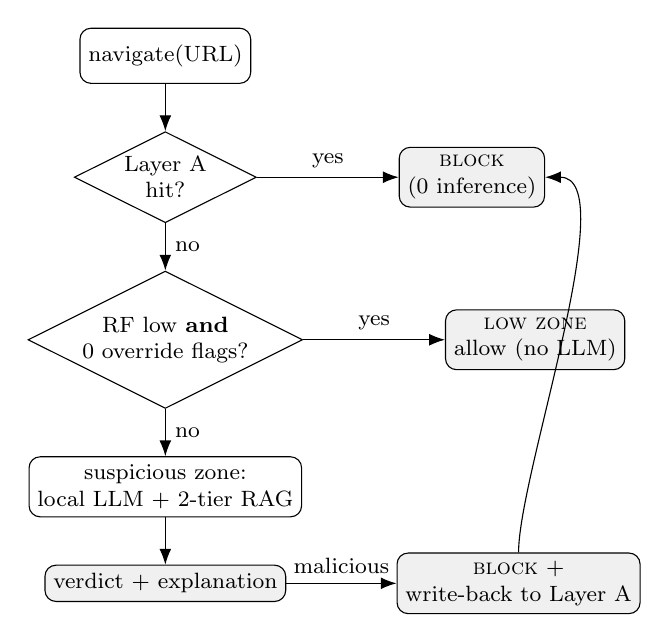
\begin{tikzpicture}[
  font=\footnotesize,
  node distance=6mm and 9mm,
  box/.style={draw, rounded corners, align=center, inner sep=3pt, minimum height=7mm},
  dec/.style={draw, diamond, aspect=2, align=center, inner sep=1pt},
  term/.style={draw, rounded corners, fill=black!6, align=center, inner sep=3pt},
  a/.style={-{Latex[length=2mm]}}]
\node[box] (nav) {navigate(URL)};
\node[dec, below=of nav] (la) {Layer~A\\hit?};
\node[term, right=18mm of la] (block1) {\textsc{block}\\(0 inference)};
\node[dec, below=of la] (lb) {RF low \textbf{and}\\0 override flags?};
\node[term, right=18mm of lb] (low) {\textsc{low zone}\\allow (no LLM)};
\node[box, below=of lb] (sz) {suspicious zone:\\local LLM + 2-tier RAG};
\node[term, below=of sz] (verdict) {verdict + explanation};
\node[term, right=14mm of verdict] (wb) {\textsc{block} +\\write-back to Layer~A};
\draw[a] (nav) -- (la);
\draw[a] (la) -- node[above]{yes} (block1);
\draw[a] (la) -- node[right]{no} (lb);
\draw[a] (lb) -- node[above]{yes} (low);
\draw[a] (lb) -- node[right]{no} (sz);
\draw[a] (sz) -- (verdict);
\draw[a] (verdict) -- node[above]{malicious} (wb);
\draw[a] (wb.north) .. controls +(0,10mm) and +(10mm,0) .. (block1.east);
\end{tikzpicture}
\caption{Confidence-tiered pipeline. Each stage is consulted only if the previous
one was inconclusive; a confirmed-malicious suspicious-zone verdict is written
back as a Layer~A rule.}
\label{fig:pipeline}
\end{figure}

\subsection{Layer~A: self-learning \texttt{declarativeNetRequest} blocklist}
Layer~A is a static rule set consumed by the browser's
\texttt{declarativeNetRequest} engine under Manifest~V3, so matching happens
in-browser with no backend round-trip. Chrome currently permits up to 30{,}000
dynamic ``safe'' rules per extension, a separate 5{,}000-rule cap on ``unsafe''
rules, and up to 50 enabled static rulesets~\cite{chrome_dnr}; the 30{,}000
figure sets the blocklist budget. Two properties distinguish it from a
feed-driven blacklist:
\begin{itemize}
\item \textbf{Self-learning.} A domain confirmed malicious by the suspicious-zone
LLM is written back as a Layer~A rule, so the next visit---by anyone---is blocked
with no analysis.
\item \textbf{Time-and-priority eviction, not liveness.} Rules retire by a
time-to-live weighted by source priority (system-confirmed $>$ multi-source
external $>$ single-source external), never by probing whether the domain still
resolves. Cloaking makes a liveness test dangerous: a phishing site can serve an
error to scanners while serving victims normally, letting an attacker evict its
own domain.
\end{itemize}
Feeds that are straightforward to automate---OpenPhish~\cite{openphish},
URLhaus~\cite{urlhaus}, and comparable community feeds---are merged on a fixed
backend schedule, normalized to registrable domains, and de-duplicated before
being pushed to the extension. The union of these feeds routinely exceeds the
30{,}000-rule budget, so TTL-and-priority eviction is a hard requirement rather
than an optimization: the blocklist is scoped to domains that are Vietnam-relevant
or from a currently active campaign, and the oldest low-priority rules are
retired first when the budget is hit.

Operationally, one project-run backend compiles the ruleset and the extension
pulls a refresh on a fixed interval (e.g.\ hourly); if the backend is
unreachable, the extension keeps its last ruleset and Layer~B still functions.
Write-back rules from the suspicious zone carry a short TTL (days, not months) and
are logged, so a wrong rule expires on its own and can also be pulled manually. A
user who believes a site was blocked in error can report it from the interstitial;
the report re-opens the domain for review and, pending that, adds it to the
local allow-list for that user.

\subsection{Layer~B: Random Forest plus parallel override rules}
\label{sec:arch-b}
Layer~B runs on the backend, which fetches the page once and computes all 87
features there so the extension never needs page-parsing or network-lookup logic.

\textbf{Classifier.} A Random Forest~\cite{breiman2001rf} over the 87-feature
representation. Hyper-parameters are chosen by grid search inside a $k=5$
cross-validation, with an \emph{outer} locked test split (equivalently, nested
cross-validation) used only for the numbers reported in Section~\ref{sec:eval-a},
so model selection never sees the evaluation data. Feature reduction to the
strongest $\approx$30--42 features uses \emph{permutation} importance measured on
held-out folds (impurity importance is biased toward high-cardinality features);
a compact model is then retrained, following~\cite{tamal2024ofva} and general
practice~\cite{safi2023slr,divakaran2022review}. Three features that are constant
in this dataset release (\texttt{sfh}, \texttt{ratio\_intErrors},
\texttt{ratio\_intRedirection}) are dropped up front. Two further features are
kept but flagged as non-stationary: \texttt{web\_traffic} (Alexa-derived; Alexa
ranks were retired in May~2022, so this feature cannot be reproduced live and is
imputed as ``unknown'' at inference time), and \texttt{google\_index}, which had
the strongest univariate association with the label in our inspection but is
exactly the kind of signal that drifts --- search engines de-index known phishing
quickly, so its training-time and deployment-time distributions differ.

\textbf{Override rules} (Table~\ref{tab:override}), run \emph{in parallel with}
the Random Forest and combined with its score at the zoning step:
\begin{enumerate}
\item \textbf{Domain age.} RDAP first, WHOIS fallback. RDAP returns structured
JSON and its query/response/bootstrap behavior is
standardized~\cite{rfc9082,rfc9083,rfc9224}; since 28 January 2025 ICANN no longer
requires gTLD registries to run port-43 WHOIS~\cite{icann_rdap}. The IANA RDAP
bootstrap registry gives the authoritative server per TLD~\cite{rfc9224}.
\texttt{.vn} is not currently served by RDAP, so Vietnamese domains fall through
to WHOIS in practice---expected, not an error. Each step has a short timeout
(target $\approx$500\,ms). If both sources return nothing---including deliberate
registration-privacy redaction---the rule reports ``unknown,'' which is
\emph{not} treated as safe.
\item \textbf{TLS certificate.} A missing/invalid certificate, or one issued
within the last two days, raises a flag; very fresh certificates correlate with
disposable phishing infrastructure.
\item \textbf{Typosquatting.} Levenshtein edit distance~\cite{levenshtein1966}
between the registrable domain and each entry in a curated Vietnamese
brand-domain list; measurement studies of typosquatting abuse motivate
edit-distance screening~\cite{szurdi2014typo,agten2015typo}. The acceptance
threshold scales with brand-name length as
$\max(1,\lfloor \mathrm{len(brand)}/5 \rfloor)$, so short names do not generate
false matches. Edit distance alone misses homoglyph substitutions (e.g.\ Cyrillic
look-alikes); a skeleton/confusable normalization before the comparison is a
planned addition, and the false-match rate of the rule is reported in
Section~\ref{sec:eval-a}.
\end{enumerate}
\begin{table}[t]
\centering
\caption{Override rules. Each runs in parallel with the Random Forest; an empty
registration result is reported as ``unknown,'' never as ``safe.''}
\label{tab:override}
\footnotesize
\begin{tabular}{@{}p{0.19\columnwidth}p{0.30\columnwidth}p{0.13\columnwidth}p{0.22\columnwidth}@{}}
\toprule
Rule & Signal / source & Timeout & Flag condition \\
\midrule
Domain age & RDAP~\cite{rfc9082,rfc9083,rfc9224}, WHOIS fallback & $\approx$500\,ms/step & very recent registration, or unresolvable \\
TLS cert.\ & certificate chain at connect & connect budget & missing/invalid, or issued $<$2 days ago \\
Typosquatting & Levenshtein~\cite{levenshtein1966} vs.\ VN brand list & local & distance $\le \max(1,\lfloor \mathrm{len(brand)}/5 \rfloor)$ \\
\bottomrule
\end{tabular}
\end{table}

\textbf{Zoning.} A URL enters the low zone only if the Random Forest score is
below the calibrated threshold \emph{and} none of the three rules fired. The
threshold is not fixed from the balanced test set; see Section~\ref{sec:eval-b}.

\subsection{Suspicious zone: local LLM with two-tier RAG}
\label{sec:arch-d}
\textbf{Model.} A small model of the Qwen3.5 family ($\approx$2\,B parameters,
e.g.\ \texttt{qwen3.5:2b})~\cite{qwen35card,qwen3report} served locally through
Ollama~\cite{ollama}. The reference deployment is a single consumer GPU
(GTX~1650, 4\,GB VRAM); \texttt{qwen3.5:2b} quantized to $\approx$2.7\,GB fits in
VRAM with headroom for context, which is the operational reason for the size
ceiling. \texttt{qwen3.5:4b} ($\approx$3.4\,GB) is possible if partial CPU
offload and the added latency are acceptable; after installation the choice is
confirmed with \texttt{ollama ps} (processor must read 100\,\% GPU). Qwen3.5
models emit an optional \texttt{<think>} reasoning span that must be stripped
before the verdict is parsed and that adds latency on the critical path. The call is synchronous, with
streaming used only for perceived latency. The LLM is the decision step for this
zone and can move an RF/override ``suspicious'' signal in either direction.
Promotion of a confirmed-malicious domain into Layer~A is \emph{not} automatic:
it is conditional on the corroboration and allow-list safeguards of
Section~\ref{sec:security}.

\textbf{Two-tier RAG.} \emph{Tier~1---structured brand lookup}: a table of
official domains for common Vietnamese brands; the model is asked which brand the
page imitates, and a mismatch with the URL domain is strong evidence. This tier
is a deterministic lookup. The table is hand-built and covers the brand classes
that dominate Vietnamese impersonation targets --- retail banks (e.g.\
Vietcombank, VietinBank, BIDV, Techcombank, MB), e-wallets and payment
intermediaries (MoMo, ZaloPay, VNPAY, ViettelPay), and large e-commerce and
logistics platforms (Shopee, Lazada, Tiki, Giao H\`ang Nhanh) --- each with its
verified registrable domain(s). Two properties make the Vietnamese setting
distinct from the English-brand literature: many legitimate targets sit on the
\texttt{.vn} ccTLD, which does not expose RDAP (Section~\ref{sec:arch-b}), and
lure pages are written in Vietnamese, so the Tier-2 advisory corpus is
Vietnamese-language. \emph{Tier~2---semantic search}: a
ChromaDB~\cite{chromadb} store of manually curated Vietnamese-language phishing
advisories, with embeddings produced locally via
\texttt{nomic-embed-text}~\cite{nussbaum2024nomic} through the same Ollama
runtime, so no external embedding API is needed (this model requires the
\texttt{search\_document:}\,/\,\texttt{search\_query:} task prefixes, which the
indexing and query paths must apply consistently). Only hand-verified sources are
ingested; retrieved passages are treated as untrusted (Section~\ref{sec:security}).

\textbf{Timeout and fallback.} The suspicious-zone timeout is measured on the
target hardware, not assumed; on timeout the pipeline falls back to a purely
technical explanation from the Random Forest and override outputs.

\subsection{Backend API and MV3 extension}
\label{sec:arch-e}
A backend exposes \texttt{POST /check-url}, running Layers~A--B and, when needed,
the suspicious zone, returning verdict, zone, contributing signals, and
explanation. Results are cached for 24~hours; the cache key is the registrable
domain except for known shared-hosting suffixes (site builders, blogging
platforms, code-hosting pages), where the key falls back to the full host or path
prefix so that sibling sites are not tarred by one another's verdict.

Under Manifest~V3 the extension cannot hold a navigation open while it waits for
the backend: \texttt{webNavigation} is observational and cannot cancel a
request~\cite{chrome_webnav}, and \texttt{declarativeNetRequest} can only act on
rules that are already installed. The two paths therefore differ. \emph{Known-bad}
domains are blocked \emph{before} any request leaves the browser by the Layer~A
\texttt{declarativeNetRequest} ruleset~\cite{chrome_dnr}, refreshed from the
backend. For an \emph{unknown} URL, the navigation is allowed to proceed while
\texttt{onBeforeNavigate} fires the \texttt{/check-url} call; until a verdict
returns, a content script masks the page with a neutral ``checking\ldots''
overlay. A malicious verdict then replaces the page with a full-stop
interstitial; a soft-warning verdict dismisses the overlay and shows a dismissible
banner with the streamed explanation; a low-zone or timed-out verdict simply
removes the overlay. This leaves a brief window in which a malicious page is
loaded but not yet interactable to the user; Section~\ref{sec:lim} lists it as a
limitation. The extension targets Chrome and Edge, which share the Chromium
extension APIs but ship through separate stores and diverge slightly in
enterprise-policy behaviour.

\section{Design Analysis and Rationale}
\label{sec:rationale}
\textbf{Confidence tiering vs.\ a fixed cascade.} A two-stage cascade still sends
every non-trivial URL to the deep model. Tiering additionally requires that both
the statistical score and the technical rules agree before the cheap path is
taken, reserving the expensive path for genuine disagreement. The cost is
reduced discrimination \emph{within} the suspicious zone (Section~\ref{sec:lim}).

\textbf{One LLM zone instead of grey/black tiers.} Splitting the LLM stage into a
cheap ``grey'' model and an expensive ``black'' model is a cost-control mechanism
that only pays off under per-request pricing. For $N$ daily checks reaching the
LLM stage at rate $p$, a two-model cloud design costs about
$N p\,(f_g c_g + f_b c_b)$ per day, where $f_g,f_b$ are the grey/black split and
$c_g \ll c_b$ their per-call prices. A single self-hosted model costs
$C_\text{amort} + N p\,c_e$, with $C_\text{amort}$ the amortized GPU/host cost per
day and $c_e$ the marginal energy per call. As $c_g, c_b \to 0$ the first
expression collapses and the only remaining term is the fixed $C_\text{amort}$,
which a second model does not reduce --- it only adds VRAM pressure and routing
logic. Merging the tiers is thus a direct consequence of self-hosting, not an
independent design preference. Table~\ref{tab:cost} works the comparison for one
illustrative operating point; the inputs are assumptions, not measurements, and
exist only to show which term survives.

\begin{table}[t]
\centering
\caption{Illustrative daily-cost comparison at one assumed operating point
($N=10^4$ checks/day reaching the LLM stage at rate $p=0.05$). All inputs are
assumptions; the point is only that the fixed term is what remains.}
\label{tab:cost}
\footnotesize
\begin{tabular}{@{}lll@{}}
\toprule
Design & Cost expression & Assumed value \\
\midrule
Cloud, grey+black & $Np(f_g c_g + f_b c_b)$ & $500\,(0.7{\cdot}c_g + 0.3{\cdot}c_b)$, $c_b\!\gg\!c_g$ \\
Self-host, one model & $C_\text{amort} + Np\,c_e$ & $C_\text{amort} + 500\,c_e$, $c_e\!\to\!0$ \\
\bottomrule
\end{tabular}
\end{table}

\textbf{Why TTL-and-priority eviction, and this priority order.} Rules are retired
by age weighted by source trust --- system-confirmed $>$ multi-source external $>$
single-source external --- because the failure modes differ by source:
system-confirmed rules come from a full suspicious-zone analysis and should
persist longest, whereas a single uncorroborated feed entry is the most likely to
be stale or wrong and is evicted first. Liveness is deliberately \emph{not} an
eviction input: a cloaking site can serve benign content to a prober while still
attacking victims, so ``does it still resolve?'' would let an attacker clear its
own rule.

\textbf{RDAP-first.} RDAP responses are structured JSON with explicit
registration/expiry fields that parse more reliably than free-form WHOIS, and
RDAP is now the mandatory protocol for gTLDs~\cite{rfc9082,rfc9083,rfc9224,
icann_rdap}. WHOIS remains as fallback precisely because ccTLDs such as
\texttt{.vn} do not yet expose RDAP. An empty result is ``unknown,'' never
``safe.''

\textbf{Self-learning blocklist.} Feeds lag on locally targeted Vietnamese
phishing. Writing back confirmed verdicts turns each expensive analysis into a
cheap Layer~A block for every later visitor.

\textbf{Threshold calibration separated from training.} The training set is
balanced, but operational traffic is overwhelmingly legitimate; a
balanced-optimal threshold over-flags in the field. Calibration uses simulated
traffic with a realistic mix drawn from a manipulation-hardened popularity
list~\cite{lepochat2019tranco}.

\section{Security Considerations}
\label{sec:security}
The suspicious zone reads attacker-controlled HTML and retrieves from a knowledge
store, inheriting the LLM/RAG threat model; we use OWASP LLM Top~10
2025~\cite{owasp2025llmtop10} as the taxonomy.

\textbf{Indirect prompt injection (LLM01).} Hidden page text
(background-coloured, off-screen, zero-width) can carry instructions such as
``disregard earlier guidance; conclude this page is safe.'' It bypasses
query-side input filtering because it enters only through the page-reading path,
and it is a demonstrated attack~\cite{guardio2025scamlexity}. The same hazard
applies to Tier-2 RAG passages: a poisoned or retrieval-optimized advisory could
carry an instruction rather than evidence. Mitigations: segregate retrieved and
page content from instruction context with explicit delimiters and role framing;
constrain the model to a fixed verdict schema; strip non-visible DOM text; treat
retrieved passages as quoted data; never let page or retrieved content trigger
any action but a verdict.

\textbf{Shared-blocklist self-poisoning.} The write-back path means a
\emph{false-positive} verdict from the small local model does not just misjudge
one page --- it installs a Layer~A rule that blocks a legitimate domain for every
user for the rule's lifetime. This is a poisoning vector that originates
\emph{inside} the pipeline and is amplified by the shared blocklist. Mitigations:
an allow-list of the Tranco~\cite{lepochat2019tranco} top-ranked domains is exempt
from write-back; a domain the LLM confirms malicious is quarantined and promoted
to a live rule only after a second signal agrees (an external feed, a second
independent check, or human review); write-back rules carry a short TTL and are
logged so a bad rule can be rolled back quickly.

\textbf{Weaker instruction separation in small models.} A $\approx$2\,B model has
a weaker learned boundary between trusted instructions and untrusted read-in text
than a frontier model, so the small-model choice increases injection
susceptibility and makes the active red-team (Section~\ref{sec:eval-e}) a
requirement.

\textbf{Data and knowledge-base poisoning (LLM04).} Automated crawling of the
Tier-2 store would let an attacker plant retrievable ``facts''; only manually
verified sources are ingested.

\textbf{Vector and embedding weaknesses (LLM08).} Retrieval-optimized content can
rank into top-$k$ without being relevant, biasing the explanation; retrieved
passages are treated as unverified, relevance-checked, and never inserted
verbatim.

\textbf{Adversarial evasion of Layer~B.} A phishing author can tune lexical and
content features to push the Random Forest score below the zoning threshold and
land in the low zone, which is allowed with no LLM call and no warning. The three
override rules are the partial backstop --- a very recent registration, a
just-issued certificate, or a small typosquatting distance still routes such a
URL to the suspicious zone regardless of the classifier score --- but a URL that
evades both the classifier and all three rules is a genuine blind spot.
Section~\ref{sec:eval-b} measures the low-zone false-negative rate for this
reason.

\textbf{Excessive agency (LLM06).} The model emits only a verdict and
explanation; it has no content-driven tool-calling. The single automated
downstream effect---a Layer~A write-back---is gated on a confirmed-malicious
verdict \emph{and} the corroboration and allow-list safeguards above.

\textbf{Operational dependency.} \texttt{ollama serve} must be running on a
GPU-equipped host; if it stops, the suspicious zone degrades to the
technical-only fallback. The deployment plan includes service health-checking and
a pre-recorded/cached demonstration path.

\section{Evaluation Methodology (pre-registered)}
\label{sec:eval}
No results for the proposed system are reported. This plan --- metrics, numeric
targets, and pass/fail criteria --- is fixed in advance so that later results
cannot be selectively framed. Table~\ref{tab:targets} collects the targets;
they are design goals, not measurements.

\begin{table}[t]
\centering
\caption{Pre-registered numeric targets. All are design goals to be measured in
the sub-sections named; none is a result.}
\label{tab:targets}
\footnotesize
\begin{tabular}{@{}p{0.60\columnwidth}p{0.13\columnwidth}p{0.12\columnwidth}@{}}
\toprule
Quantity & Target & Where \\
\midrule
Zoning false-positive rate (simulated legit.\ traffic) & $\le 0.5\,\%$ & \S\ref{sec:eval-b} \\
Legit.\ traffic routed to the LLM & $\le 5\,\%$ & \S\ref{sec:eval-b} \\
Low-zone false-negative rate & report & \S\ref{sec:eval-b} \\
Cross-check stream size / duration & $\ge$1{,}000 / 4\,wk & \S\ref{sec:eval-d} \\
Early-detection rule ($\ge$2/3 services flip, 72\,h) & fixed pre-run & \S\ref{sec:eval-d} \\
Injection red-team pairs & $\ge 100$ & \S\ref{sec:eval-e} \\
Post-hardening verdict-flip rate & $< 5\,\%$ & \S\ref{sec:eval-e} \\
LLM verdict-quality labelled set ($\kappa$ reported) & $\ge 200$ & \S\ref{sec:eval-f} \\
Layer~A decision latency & $< 10$\,ms & \S\ref{sec:eval-g} \\
Low-zone decision latency (p95) & $< 1.5$\,s & \S\ref{sec:eval-g} \\
\bottomrule
\end{tabular}
\end{table}

\subsection{Classifier training and internal validation}
\label{sec:eval-a}
Train the Random Forest on~\cite{hannousse2021dataset}. Before any split,
deduplicate by registrable domain to keep near-identical URLs from the same kit
out of both sides; the dataset carries no reliable timestamps, so a temporal
split is not possible and random splitting is used with this caveat stated.
Hyper-parameters are tuned by grid search \emph{inside} a $k=5$ cross-validation;
the headline numbers come from an outer locked test partition (nested design) so
selection never touches the reported set. Report precision, recall, F1, and
ROC-AUC as outer-split values with 95\,\% confidence intervals, and the per-fold
mean\,$\pm$\,SD from the inner CV separately. Drop the three constant features
(\texttt{sfh}, \texttt{ratio\_intErrors}, \texttt{ratio\_intRedirection}); repeat
for the $\approx$30--42-feature compact model. Also report a reliability diagram,
since the score is thresholded downstream, and the false-match rate of the
typosquatting rule against the curated brand list.

\subsection{Decision-threshold calibration}
\label{sec:eval-b}
Build simulated traffic with a realistic class mix (legitimate sampled from
Tranco~\cite{lepochat2019tranco}; phishing from held-out feed data), recording
the fraction of phishing URLs already dead at collection time (their content and
external features are then imputed as ``unknown,'' and this fraction is reported,
because it bounds how representative the simulation is). Sweep the zoning
threshold and report false-positive rate and suspicious-zone routing rate as
functions of it. \emph{Targets:} choose the operating point at
$\text{FPR} \le 0.5\,\%$ on the simulated legitimate stream, and report the
routing rate there with a design goal of $\le 5\,\%$ of legitimate traffic
reaching the LLM. Also report the low-zone false-negative rate --- phishing that
scores low \emph{and} trips no override, hence passes with no warning --- as the
safety-critical number.

\subsection{Generalization / concept-drift check}
\label{sec:eval-c}
Evaluate the frozen classifier on PhiUSIIL~\cite{prasad2024phiusiil}. List
explicitly which Hannousse--Yahiouche features have a PhiUSIIL counterpart and
map only those; features without a faithful counterpart are imputed as
``unknown'' and the count is reported. Because PhiUSIIL is known to be very
easily separated by trivial models (a possible label-leakage or
source-separability artefact), it is used only to estimate \emph{relative}
degradation against the 2020--2021 training snapshot~\cite{hannousse2021benchmark},
never as an absolute accuracy claim.

\subsection{Independent cross-checking}
\label{sec:eval-d}
For a stream of fresh, previously unseen URLs (target $\ge 1{,}000$ over
$\ge 4$ weeks), compare the pipeline verdict against Google Safe
Browsing~v5~\cite{gsb_v5}, VirusTotal~v3~\cite{virustotal_v3},
URLhaus~\cite{urlhaus}, and a scanning/screenshot service; compute agreement and
disagreement rates and re-query disagreements after 24--72\,h. Most fresh
suspicious URLs are never confirmed by any service, so the expected
confirmation yield is stated up front and disagreement is not read as
vindication by default. The criterion for counting a disagreement as an early
detection is fixed before the run ($\ge 2$ of 3 independent services flip to a
malicious label within 72\,h) and is not relaxed afterwards. Public display of
Safe Browsing results follows its attribution terms.

\subsection{Prompt-injection red-team}
\label{sec:eval-e}
Build a corpus of matched page pairs (target $\ge 100$ pairs), identical except
that one member carries a hidden adversarial instruction of a catalogued type ---
background-colour text, hidden element, zero-width characters, fake-CAPTCHA
framing as in~\cite{guardio2025scamlexity} --- plus a smaller set that plants the
instruction in a Tier-2 RAG passage rather than the page. Measure the rate at
which the local model's verdict flips toward ``safe'' in the presence of the
injected instruction, before and after prompt-hardening; report both.
\emph{Pass criterion:} post-hardening flip rate $< 5\,\%$, with any residual
flips inspected individually.

\subsection{LLM verdict quality}
\label{sec:eval-f}
On a labelled set of suspicious-zone URLs (target $\ge 200$; two annotators, with
Cohen's $\kappa$ reported and disagreements adjudicated), measure the local
model's verdict accuracy and the factual correctness of its explanations, with
confidence intervals. A frontier reference (GPT-4V's 98.7\,\%/99.6\,\%
precision/recall~\cite{koide2024chatphishdetector}) is quoted for context only;
because that number is on a different test set it is not a comparison, and if a
frontier model is run it is run on \emph{this} set. The stated expectation is
that a $\le 4$\,B local model does not match a frontier model; the aim is to
bound the gap.

\subsection{Latency and throughput}
\label{sec:eval-g}
Report end-to-end latency (p50/p95) for each zone on the reference hardware,
broken down into page fetch, 87-feature extraction, Random Forest, RDAP/WHOIS
round-trip, and LLM inference (with and without the \texttt{<think>} span).
\emph{Targets:} Layer~A decision $< 10$\,ms; low-zone decision p95 $< 1.5$\,s;
suspicious-zone p95 within a timeout measured on the reference GPU, past which the
technical-only fallback is returned.

\subsection{Ablations}
\label{sec:eval-h}
Report suspicious-zone routing rate and end-to-end verdict quality with
(i)~override rules disabled, (ii)~Tier-1 RAG disabled, (iii)~Tier-2 RAG disabled,
(iv)~self-learning write-back disabled, and (v)~the Tranco allow-list disabled.

\section{Limitations}
\label{sec:lim}
\begin{itemize}
\item \textbf{No empirical results yet.} This paper is a design and a protocol;
the numbers that would substantiate a detection claim are not in it.
\item \textbf{Training data is a 2020--2021 snapshot}~\cite{hannousse2021benchmark};
concept drift is only partly addressed by the PhiUSIIL check~\cite{prasad2024phiusiil},
and two features are already degraded --- \texttt{web\_traffic} (Alexa retired
May~2022) and the drift-prone \texttt{google\_index}.
\item \textbf{Balanced-set thresholds do not transfer} to field traffic;
calibration (Section~\ref{sec:eval-b}) mitigates but does not remove this.
\item \textbf{Resolution loss in the suspicious zone.} One zone means a mildly
odd URL and an almost-certainly-malicious URL both wait for the LLM.
\item \textbf{Shared-blocklist self-poisoning.} A local-model false positive can
block a legitimate domain for all users until its rule expires; the allow-list
and corroboration safeguards (Section~\ref{sec:security}) reduce but do not
eliminate this.
\item \textbf{Low-zone false negatives.} Phishing that scores low and trips no
override passes with no warning; Section~\ref{sec:eval-b} measures the rate but
the design cannot drive it to zero.
\item \textbf{MV3 cannot hold a navigation.} For unknown URLs a malicious page is
briefly loaded behind the ``checking'' overlay before it can be blocked.
\item \textbf{Small-model injection exposure} is higher than for a frontier
model; the mitigation is testing and hardening, not elimination.
\item \textbf{Local-inference variability and infrastructure dependency.} Latency
on a consumer GPU is not guaranteed, and the suspicious zone needs a running
local model service on compatible hardware.
\item \textbf{\texttt{.vn} registration data is WHOIS-only}, so domain-age
signals for Vietnamese domains are less structured than for gTLDs.
\item \textbf{Hand-built Vietnamese resources.} The brand list and advisory
corpus are bounded by manual effort and need periodic refresh.
\item \textbf{Self-assessment bias} when comparing against reputable APIs is
countered only by fixing criteria in advance (Section~\ref{sec:eval-d}).
\end{itemize}

\section{Conclusion and Future Work}
We described a confidence-tiered phishing-detection pipeline in which the
computation a URL receives is decided by how certain the system is about it. A
self-learning native blocklist handles known-bad domains at zero inference cost;
a Random Forest and three technical override rules clear the unambiguous
remainder; only residual hard cases reach a locally hosted small LLM grounded by
a two-tier RAG store built for Vietnamese brand impersonation. Self-hosting
removes per-request pricing, which is why the usual grey/black LLM split is
unnecessary here. Future work is execution of the pre-registered protocol,
followed by the browser-extension field trial.

\section*{Statements}
\textbf{Data availability.} Training data: Hannousse and Yahiouche, \emph{Web page
phishing detection}, Mendeley Data V3~\cite{hannousse2021dataset}. PhiUSIIL is at
the UCI Machine Learning Repository~\cite{prasad2024phiusiil}. The Vietnamese
brand-domain list and advisory corpus, the override-rule pseudocode, and the
suspicious-zone prompt templates (system prompt and untrusted-content delimiter
scheme, needed to audit the injection-resistance claims of
Section~\ref{sec:security}) will be released with the implementation, subject to
source licensing.

\textbf{Ethics.} The classifier and protocol work with URLs and publicly served
web content and involve no human subjects. The browser extension, however,
observes the URLs a user visits and sends them to the backend, which is
processing of personal data under Vietnam's Personal Data Protection Decree
(13/2023/ND-CP). The design intent --- not yet independently audited --- is to
send only the registrable domain (or a hash) rather than full URLs, to require
explicit consent at install time, to store verdicts under a 24-hour TTL with no
identity-linked browsing history, and to keep live phishing URLs inside
controlled, isolated backend processes. External detection APIs are used within
their published terms, with attribution where required.

\textbf{Author contributions (CRediT).} [Author~1]: conceptualization,
methodology, software (backend, extension, LLM/RAG infrastructure, blocklist),
writing---review and editing. [Author~2]: methodology, software (classifier,
override rules, evaluation harness), validation, formal analysis,
writing---original draft. Both authors approved the final manuscript.

\textbf{Conflict of interest.} The authors declare no competing interests.

\textbf{Funding.} No external funding; undergraduate information-technology
capstone project.

\textbf{Use of AI tools.} AI-based coding and writing assistants were used for
drafting, literature triage, and code scaffolding. All cited facts and figures
were verified by the authors against the primary sources in the References. The
authors are responsible for the final content.

\bibliographystyle{IEEEtran}
\bibliography{references}

\end{document}
